% Options for packages loaded elsewhere
\PassOptionsToPackage{unicode}{hyperref}
\PassOptionsToPackage{hyphens}{url}
\PassOptionsToPackage{dvipsnames,svgnames,x11names}{xcolor}
%
\documentclass[
  12pt,
]{article}
\usepackage{amsmath,amssymb}
\usepackage{lmodern}
\usepackage{iftex}
\ifPDFTeX
  \usepackage[T1]{fontenc}
  \usepackage[utf8]{inputenc}
  \usepackage{textcomp} % provide euro and other symbols
\else % if luatex or xetex
  \usepackage{unicode-math}
  \defaultfontfeatures{Scale=MatchLowercase}
  \defaultfontfeatures[\rmfamily]{Ligatures=TeX,Scale=1}
\fi
% Use upquote if available, for straight quotes in verbatim environments
\IfFileExists{upquote.sty}{\usepackage{upquote}}{}
\IfFileExists{microtype.sty}{% use microtype if available
  \usepackage[]{microtype}
  \UseMicrotypeSet[protrusion]{basicmath} % disable protrusion for tt fonts
}{}
\makeatletter
\@ifundefined{KOMAClassName}{% if non-KOMA class
  \IfFileExists{parskip.sty}{%
    \usepackage{parskip}
  }{% else
    \setlength{\parindent}{0pt}
    \setlength{\parskip}{6pt plus 2pt minus 1pt}}
}{% if KOMA class
  \KOMAoptions{parskip=half}}
\makeatother
\usepackage{xcolor}
\usepackage[margin=1in]{geometry}
\usepackage{longtable,booktabs,array}
\usepackage{calc} % for calculating minipage widths
% Correct order of tables after \paragraph or \subparagraph
\usepackage{etoolbox}
\makeatletter
\patchcmd\longtable{\par}{\if@noskipsec\mbox{}\fi\par}{}{}
\makeatother
% Allow footnotes in longtable head/foot
\IfFileExists{footnotehyper.sty}{\usepackage{footnotehyper}}{\usepackage{footnote}}
\makesavenoteenv{longtable}
\usepackage{graphicx}
\makeatletter
\def\maxwidth{\ifdim\Gin@nat@width>\linewidth\linewidth\else\Gin@nat@width\fi}
\def\maxheight{\ifdim\Gin@nat@height>\textheight\textheight\else\Gin@nat@height\fi}
\makeatother
% Scale images if necessary, so that they will not overflow the page
% margins by default, and it is still possible to overwrite the defaults
% using explicit options in \includegraphics[width, height, ...]{}
\setkeys{Gin}{width=\maxwidth,height=\maxheight,keepaspectratio}
% Set default figure placement to htbp
\makeatletter
\def\fps@figure{htbp}
\makeatother
\setlength{\emergencystretch}{3em} % prevent overfull lines
\providecommand{\tightlist}{%
  \setlength{\itemsep}{0pt}\setlength{\parskip}{0pt}}
\setcounter{secnumdepth}{5}
\newlength{\cslhangindent}
\setlength{\cslhangindent}{1.5em}
\newlength{\csllabelwidth}
\setlength{\csllabelwidth}{3em}
\newlength{\cslentryspacingunit} % times entry-spacing
\setlength{\cslentryspacingunit}{\parskip}
\newenvironment{CSLReferences}[2] % #1 hanging-ident, #2 entry spacing
 {% don't indent paragraphs
  \setlength{\parindent}{0pt}
  % turn on hanging indent if param 1 is 1
  \ifodd #1
  \let\oldpar\par
  \def\par{\hangindent=\cslhangindent\oldpar}
  \fi
  % set entry spacing
  \setlength{\parskip}{#2\cslentryspacingunit}
 }%
 {}
\usepackage{calc}
\newcommand{\CSLBlock}[1]{#1\hfill\break}
\newcommand{\CSLLeftMargin}[1]{\parbox[t]{\csllabelwidth}{#1}}
\newcommand{\CSLRightInline}[1]{\parbox[t]{\linewidth - \csllabelwidth}{#1}\break}
\newcommand{\CSLIndent}[1]{\hspace{\cslhangindent}#1}
\usepackage{setspace} \setstretch{1.15} \usepackage{float} \floatplacement{figure}{t}
\ifLuaTeX
  \usepackage{selnolig}  % disable illegal ligatures
\fi
\IfFileExists{bookmark.sty}{\usepackage{bookmark}}{\usepackage{hyperref}}
\IfFileExists{xurl.sty}{\usepackage{xurl}}{} % add URL line breaks if available
\urlstyle{same} % disable monospaced font for URLs
\hypersetup{
  colorlinks=true,
  linkcolor={cyan},
  filecolor={Maroon},
  citecolor={Blue},
  urlcolor={cyan},
  pdfcreator={LaTeX via pandoc}}

\title{~\Large Increased sexual dimorphism does not evolve in a fossil
stickleback following ecological release from fish piscivores}
\author{\large Matthew Stuart\(^{1,2}\), Allison Ozark\(^{3}\), Raheyma
Siddiqui\(^3\), Akhil Ghosh\(^{1,2}\)\\
\large Samantha Swank\(^3\), Michael A. Bell\(^4\), Gregory J.
Matthews\(^{1,2}\), and Yoel E. Stuart\(^{3,+}\)\\
\vspace{-1.1mm}\\
\large \(^1\) Department of Mathematics and Statistics, Loyola
University Chicago, Chicago, IL, USA \vspace{-1.1mm}\\
\large \(^2\) Center for Data Science and Consulting, Loyola University
Chicago, Chicago, IL, USA \vspace{-1.1mm}\\
\large \(^3\) Department of Biology, Loyola University Chicago, Chicago,
IL, USA \vspace{-1.1mm}\\
\large \(^4\) University of California Museum of Paleontology, Berkeley,
CA, USA \vspace{-1.1mm}\\
\large \(^+\) Corresponding:
\href{mailto:ystuart@luc.edu}{\nolinkurl{ystuart@luc.edu}}
\vspace{-1.1mm}}
\date{}

\begin{document}
\maketitle
\begin{abstract}
Theory suggests that populations should expand their habitat- and
resource-use niches when they are freed from interactions with
competitors and predators--so-called ecological release. One way that
this ecological release can manifest is through increased differences
between males and females of the same species as they diverge into
different niches. If divergent niche use drives corresponding divergent
adaptation in in the traits used to exploit the divergent niches, then
theory predicts an increase in sexual dimorphism for those traits,
sometimes called character displacement between the sexes. Using a
dataset of 16 traits collected from 18 temporal samples spread across
16,500 years of evolution of the fossil stickleback fish,
\emph{Gasterosteus doryssus}, we tested the prediction that release from
predation inferred in this system would result in character displacement
between the sexes. We used data from populations of extant stickleback
(\emph{Gasterosteus aculeatus}) to build an imputation model to classify
individual sex in fossil specimens. Then, we quantified the extent of
sexual dimorphism at each temporal sample, and tracked how it changed
through time. NEED TO FINISH THIS \vspace{2mm}\\
\emph{Keywords}: character displacement, character release, evolutionary
time series, \emph{Gasterosteus doryssus}, missing data imputation
\end{abstract}

\newcommand{\iid}{\overset{iid}{\sim}}

\newpage

\hypertarget{sec:intro}{%
\section{Introduction}\label{sec:intro}}

Ecological release theory suggests that a population's niche should
change when important species interactions like resource competition or
predation are relaxed or removed (reviewed in Herrmann, Stroud, and
Losos (\protect\hyperlink{ref-Herrmannetal2021}{2021})). Removal is
posited to create ecological opportunity---i.e., aspects of the niche
become newly accessible, and the focal population shifts and/or expands
its resource use new resources (Parent and Crespi
(\protect\hyperlink{ref-ParentandCrespi2009}{2009}); Herrmann, Stroud,
and Losos (\protect\hyperlink{ref-Herrmannetal2021}{2021})). Ecological
release may then be followed by adaptive morphological evolution as
traits change to reflect the new niche (Parent and Crespi
(\protect\hyperlink{ref-ParentandCrespi2009}{2009}); Herrmann, Stroud,
and Losos (\protect\hyperlink{ref-Herrmannetal2021}{2021})).

For example, a population undergoing ecological release can experience
disruptive selection on males and females stemming from intraspecific
competition over newly accessible resources (Bolnick and Doebeli
(\protect\hyperlink{ref-BolnickandDoebeli2003}{2003}); Bolnick and Lau
(\protect\hyperlink{ref-BolnickandLau2008}{2008}); Cooper, Gilman, and
Boughman (\protect\hyperlink{ref-Cooperetal2011}{2011})). This is
predicted to result in intersexual divergence in habitat use and
associated phenotypes (Schoener
(\protect\hyperlink{ref-Schoener1968}{1968}); Shine
(\protect\hyperlink{ref-Shine1989}{1989}); Bolnick and Doebeli
(\protect\hyperlink{ref-BolnickandDoebeli2003}{2003}); Butler and Losos
(\protect\hyperlink{ref-Butleretal2007}{2007}); Bolnick and Lau
(\protect\hyperlink{ref-BolnickandLau2008}{2008}); Cooper, Gilman, and
Boughman (\protect\hyperlink{ref-Cooperetal2011}{2011}); but see Stuart
et al. (\protect\hyperlink{ref-Stuartetal2021}{2021}); Blain
(\protect\hyperlink{ref-Blain2022}{2022})). Such competition-driven
``intraspecific character displacement'' between the sexes is therefore
one explanation for the evolution of sexual dimorphism (Pfennig and
Pfennig (\protect\hyperlink{ref-PfennigandPfennig2012}{2012}); De Lisle
and Rowe (\protect\hyperlink{ref-DeLisleandRowe2015}{2015}); De Lisle
and Rowe (\protect\hyperlink{ref-DeLisleandRowe2017}{2017}), De Lisle,
Paiva, and Rowe (\protect\hyperlink{ref-DeLisleetal2018}{2018})).

Much of the theory and empirical data for character displacement between
the sexes is based on release from resource competition specifically
(e.g., Bolnick and Doebeli
(\protect\hyperlink{ref-BolnickandDoebeli2003}{2003}); Cooper, Gilman,
and Boughman (\protect\hyperlink{ref-Cooperetal2011}{2011}); Pfennig and
Pfennig (\protect\hyperlink{ref-PfennigandPfennig2012}{2012}); De Lisle
and Rowe (\protect\hyperlink{ref-DeLisleandRowe2015}{2015}); De Lisle,
Paiva, and Rowe (\protect\hyperlink{ref-DeLisleetal2018}{2018})).
However, release from predation might also drive the evolution of
increased sexual dimorphism because an absence of predators should
generate ecological opportunity (Reimchen and Nosil
(\protect\hyperlink{ref-ReimchenandNosil2004}{2004}); Parent and Crespi
(\protect\hyperlink{ref-ParentandCrespi2009}{2009}); Herrmann, Stroud,
and Losos (\protect\hyperlink{ref-Herrmannetal2021}{2021})).

Here, we tested the prediction that a release from predation results in
the evolution of increased sexual dimorphism using a well-preserved,
finely-resolved sequence of a fossil threespine stickleback fish
(Gasterosteus doryssus). The sequence in this depositional environment
is comprised of two lineages (Bell
(\protect\hyperlink{ref-Bell2009}{2009}); Cerasoni, Bell, and Stuart
(\protect\hyperlink{ref-Cerasonietal2024}{2024})). Lineage I was a
low-armor form with zero to one dorsal spines and highly reduced
pelvises, on average. Lineage I lasted for at least 93,000 years before
it was replaced by a second lineage, suddenly, likely on the order of
years (Bell, Baumgartner, and Oslon
(\protect\hyperlink{ref-Belletal1985}{1985}); Stuart et al.~unpublished
data). Lineage II appeared in the depositional environment fully
armored, with complete pelvic girdles, two pelvic spines, and three
dorsal spines (Bell, Travis, and Blouw
(\protect\hyperlink{ref-Belletal2006}{2006}); Stuart, Travis, and Bell
(\protect\hyperlink{ref-Stuartetal2020}{2020})). It then immediately
began evolving adaptive reduction in its armor traits (Hunt, Bell, and
Travis (\protect\hyperlink{ref-Huntetal2008}{2008}); Stuart, Travis, and
Bell (\protect\hyperlink{ref-Stuartetal2020}{2020})) until it reached
the same low-armor state previously held by lineage I.

The observation of 93,000 years of low-armor stasis in lineage I (Bell,
Baumgartner, and Oslon (\protect\hyperlink{ref-Belletal1985}{1985})) and
the observation of rapid evolution of armor loss by lineage II, both
suggest that this depositional environment lacked piscivorous fish like
trout and other salmonids known to prey on modern threespine
stickleback. Armor presence in extant threespine stickleback
(Gasterosteus aculeatus) correlates strongly with the presence of
vertebrate piscivores; populations with less predation pressure
typically have less armor (Reimchen
(\protect\hyperlink{ref-Reimchen1994}{1994}), Reimchen and Nosil
(\protect\hyperlink{ref-ReimchenandNosil2004}{2004}); Bell et al.
(\protect\hyperlink{ref-Belletal1993}{1993}); Roesti et al.
(\protect\hyperlink{ref-Roestietal2023}{2023})). In our paleolake basin,
only three fossil trout have been found in the same section of rock that
has revealed \textgreater20,000 threespine stickleback fossils as well
as occasional killifish (Fundulus nevadensis) (Bell
(\protect\hyperlink{ref-Bell2009}{2009}); Cerasoni, Bell, and Stuart
(\protect\hyperlink{ref-Cerasonietal2024}{2024})). Thus, we reconstruct
an evolutionar history in which it is likely that lineage II migrated
from a nearby paleolake basin that had predators since it was armored
when it arrived (Bell (\protect\hyperlink{ref-Bell2009}{2009});
Cerasoni, Bell, and Stuart
(\protect\hyperlink{ref-Cerasonietal2024}{2024})). Lineage II then
experienced release from predators in the focal paleolake basin,
generating the initial conditions of evolutionary models predicting the
evolution of increased sexual dimorphism following ecological release.
We test this prediction here.

A major challenge in the study of fossilized sexual dimorphism is
assigning sex to individual specimens in the first place (Hone and
Mallon (\protect\hyperlink{ref-HoneandMallon2017}{2017}); Mallon
(\protect\hyperlink{ref-Mallon2017}{2017}); Saitta et al.
(\protect\hyperlink{ref-Saittaetal2020}{2020})). This typically cannot
be done directly, except for taxa whose sexes are distinguished by the
presence or absence of sex-specific characters that preserve well.
Instead, paleobiologists often resort to statistical detection of sex
and sexual dimorphism, including tests for normality and bimodality in
trait distributions (e.g., Mallon
(\protect\hyperlink{ref-Mallon2017}{2017})), mixture modeling (e.g.,
Mallon (\protect\hyperlink{ref-Mallon2017}{2017})), divergence in growth
curves (e.g., Saitta et al.
(\protect\hyperlink{ref-Saittaetal2020}{2020})), and emphasis on effect
size statistics rather than significance testing (e.g., Saitta et al.
(\protect\hyperlink{ref-Saittaetal2020}{2020})). However, dimorphic
signal can be masked by noise introduced by factors both biological and
artifactual, including extended growth during ontogeny, age-based bias
in survivorship, small sample sizes, time averaging, and taphonomic bias
(Godfrey, Lyon, and Sutherland
(\protect\hyperlink{ref-Godfreyetal1993}{1993}); Koscinski and
Pietraszewski
(\protect\hyperlink{ref-KoscinskiandPietraszewski2004}{2004}); Hone and
Mallon (\protect\hyperlink{ref-HoneandMallon2017}{2017}); reviewed in
Mallon (\protect\hyperlink{ref-Mallon2017}{2017}); reviewed in Saitta et
al. (\protect\hyperlink{ref-Saittaetal2020}{2020})). Thus, the best
approach to sex classification is likely one of total evidence (Saitta
et al. (\protect\hyperlink{ref-Saittaetal2020}{2020})), including
comparison to closely-related, extant species of known sex (e.g., Hone
and Mallon (\protect\hyperlink{ref-HoneandMallon2017}{2017}); Saitta et
al. (\protect\hyperlink{ref-Saittaetal2020}{2020})).

For our study, we inferred sex in G. doryssus fossils by comparing
multivariate morphological trait data from lineage II samples to the
same multivariate trait set collected from multiple populations in the
closely-related, extant Threespine Stickleback species complex
(Gasterosteus aculeatus). Crucially, we determined G. aculeatus sex
directly via dissection and/or PCR genotyping. This enabled us to use
Multiple Imputation by Chained Equations (MICE; Buuren and
Groothuis-Oudshoorn (\protect\hyperlink{ref-MICE}{2011})) to build a
predictive multiple imputation algorithm (Little and Rubin
(\protect\hyperlink{ref-little2002statistical}{2002})) based on the
multivariate morphology of G. aculeatus individuals of known sex. We
applied this algorithm to the fossil data to impute individual sex based
on morphology, treating fossil sex as a missing variable. With sex
assigned to fossil specimens, we fit a modified Ornstein-Uhlenbeck (OU)
(Uhlenbeck and Ornstein (\protect\hyperlink{ref-OUProcess}{1930})) model
using a Bayesian framework that accounts for uncertainty in sex
classification to test for evolution of sexual dimorphism in each trait
over \textasciitilde16,000 years of lineage II.

\hypertarget{sec:data}{%
\section{Data}\label{sec:data}}

\hypertarget{fossil-specimen-data}{%
\subsection{Fossil Specimen Data}\label{fossil-specimen-data}}

We used Gasterosteus doryssus data that were previously reported by
Stuart, Travis, and Bell (\protect\hyperlink{ref-Stuartetal2020}{2020}),
Voje, Bell, and Stuart (\protect\hyperlink{ref-Vojeetal2022}{2022}), and
Siddiqui et al. (\protect\hyperlink{ref-Siddiquietal2024}{2024}).
Briefly, the data were collected from fossil Series K from Quarry D
(Cerasoni, Bell, and Stuart
(\protect\hyperlink{ref-Cerasonietal2024}{2024})), dug from an open pit
diatomite mine at 9.526° N, 119.094° W, near Hazen, Nevada, USA. Series
K consisted of 18 samples taken at \textasciitilde1000-year intervals,
and mean sample times span \textasciitilde16,363 years. Fish from series
K were measured for 16 ecomorphological traits related to armor,
swimming, and feeding (Table 1). Series K started at the previously
documented horizon when lineage I was replaced by lineage II. The tempo
and mode of lineage II armor reduction during this sequence suggests
adaptive evolution by natural selection (Hunt, Bell, and Travis
(\protect\hyperlink{ref-Huntetal2008}{2008})), and we focus on the
multivariate evolution of sexual dimorphism by this second lineage.

The lineage II fossil data consist of 814 specimens of unknown sex
sampled across the 18 K series samples. Figure 1 shows the sample size
for each of the 18 samples. There are at least 22 specimens in each
sample with a high of 67 specimens in sample 7.

\begin{longtable}[]{@{}
  >{\raggedright\arraybackslash}p{(\columnwidth - 4\tabcolsep) * \real{0.2034}}
  >{\raggedright\arraybackslash}p{(\columnwidth - 4\tabcolsep) * \real{0.0847}}
  >{\raggedright\arraybackslash}p{(\columnwidth - 4\tabcolsep) * \real{0.7119}}@{}}
\toprule()
\begin{minipage}[b]{\linewidth}\raggedright
Trait Name
\end{minipage} & \begin{minipage}[b]{\linewidth}\raggedright
Trait Code
\end{minipage} & \begin{minipage}[b]{\linewidth}\raggedright
Trait Description
\end{minipage} \\
\midrule()
\endhead
Standard Length & \texttt{stl} & Distance from anterior tip of
premaxilla to posterior end of last vertebra (i.e., the llhypural
plate) \\
Dorsal Spine Count & \texttt{mds} & Number of dorsal spines \\
Dorsal Fin Ray Count & \texttt{mdf} & Number of bones in the dorsal fin
posterior to the third dorsal spine (i.e., soft dorsal fin rays) \\
Anal Fin Ray Count & \texttt{maf} & Number of bones in the anal fin
posterior to the anal spine (i.e., soft anal fin rays) \\
Abdominal Vertebra Count & \texttt{mav} & Number of vertebrae anterior
to the first vertebra contacting an anal fin pterygiophore (Aguirre et
al.~2014) \\
Caudal Vertebra Count & \texttt{mcv} & Vertebrae including and posterior
to the first that contacts an anal fin pterygiophore (Aguirre et
al.~2014) \\
Pterygiophore Count & \texttt{mpt} & Number of pterygiophores anterior
to but excluding the pterygiophore under the third dorsal spine \\
Pelvic Spine Length & \texttt{lps.sc} & Length from the base of one
pelvic spine at its pelvic girdle articulation to its distal tip \\
Ectocoracoid Length & \texttt{ect.sc} & Length from the anterior to
posterior tips of the shoulder girdle base \\
Pelvic Girdle Length & \texttt{tpg.sc} & Length from the anterior to
posterior tips along midline. If vestigial, the sum of longest axis
along vestiges \\
Cleithrum Length & \texttt{cle.sc} & Length from dorsal tip to ventral
tip on the anterior margin of the shoulder girdle \\
Premaxilla Length & \texttt{pmx.sc} & Length from the anterior tip of
the premaxilla to the distal tip of its ascending process \\
Dorsal Spine Length & \texttt{Ds\#.sc\ \#=1/2/3} & Length from the
dorsal spine base at the pterygiophore to its distal tip \\
Pterygiophore Length & \texttt{lpt.sc} & Distance from anterior to
posterior edges of the pterygiophore immediately before ds3 (when
present) \\
\bottomrule()
\end{longtable}

\textcolor{red}{This table caption should be part of the table. Top row. at the very least, it should be the width of the table. -YS}
Table: Traits and trait descriptions. `sc' denotes size correction of
trait against standard length. Names of bones follow Bowne
(\protect\hyperlink{ref-Bowne1994}{1994}) unless otherwise noted.

\hypertarget{extant-specimen-data}{%
\subsection{Extant Specimen data}\label{extant-specimen-data}}

To span the gamut of stickleback diversity for our predictive imputation
model, we sampled modern stickleback from lakes containing generalist
stickleback populations (Hendry et al.
(\protect\hyperlink{ref-Hendryetal2009}{2009}); Bolnick
(\protect\hyperlink{ref-Bolnick2011}{2011})) and from lakes containing
benthic-limnetic species pairs (Baumgartner, Bell, and Weinberg
(\protect\hyperlink{ref-Baumgartneretal1988}{1988}); Schluter and
McPhail (\protect\hyperlink{ref-SchluterandMcPhail1992}{1992})). The
generalist specimens used here were collected by YES in 2013 and were
previously described in Stuart et al.
(\protect\hyperlink{ref-Stuartetal2017}{2017}) (Table S1). These samples
were fixed in formalin, then stained for bone with Alizarin Red in 2013.
Benthic and limnetic specimens were kindly loaned by D. Schluter and S.
Blain at the University of British Columbia. The Schluter lab collected
benthic and limnetic individuals from Enos Lake in 1988 and from Emily
Lake, Little Quarry Lake, Paxton Lake, and Priest Lake in 2018 (Table
S1). The Enos specimens had been fixed whole in formalin and stored in
40\% isopropanol. The specimens from the other lakes were initially
preserved whole in 95\% ethanol in the field before being gradually
transferred to water then formalin in the lab and ultimately stored in
40\% isopropanol. In 2019, we stained these specimens for bone using
Alizarin Red.

We next replicated fossil data collection (Table 1) on these extant
specimens. Standard length as well as pelvic-spine length on each side
were measured with calipers. We used a dissection microscope to count
dorsal spines, pelvic spines, dorsal-fin rays, and anal-fin rays. Right
and left-side pelvic girdle lengths and ectocoracoid lengths were
measured from ventral photographs taken using a Canon EOS Rebel T7 with
a Tamron 16-300 mm MACRO lens mounted on a leveled Kaiser RS1 copy
stand. Specimens were held in place for ventral photographs using a
small tabletop vise with an attached scale bar. Lateral X-rays were used
to measure dorsal spine length, number of pterygiophores anterior to the
pterygiophore holding the third spine, length of the pterygiophore just
anterior to the third spine, cleithrum length, and pre-maxilla ascending
branch length. We also counted vertebrae from the X-rays: abdominal
vertebrae were counted anterior to the first vertebra with a haemal
spine contacting an anal fin pterygiophore. Caudal vertebrae were
posterior, including the first vertebra with the haemal spine contacting
the anal fin pterygiophore (following Aguirre, Walker, and Gideon
(\protect\hyperlink{ref-Aguirreetal2014}{2014})). X-rays were taken with
an AXR Hot Shot X-ray Machine (Associated X-ray Corporation) at the
Field Museum of Natural History. Specimens were exposed at 35kV and 4mA.
Small fish were exposed for 7s, medium fish for 8s, and large fish for
10s. We developed the film and scanned individual images of each fish
using the B\&W Negatives setting on an Epson Perfection 4990 Photo
flatbed at 2400 dpi. Measurements from photographs and X-rays were taken
with FIJI (Schindelin et al.
(\protect\hyperlink{ref-Schindelinetal2012}{2012})) and its plugin
ObjectJ (\url{https://sils.fnwi.uva.nl/bcb/objectj/}). We dissected
individuals from the generalist populations (Table S1) to determine sex
from the gonads. Individuals from the species-pair lakes (TableS1) were
previously sexed by the Schluter lab, using either dissection or a
genotyping protocol \textcolor{red}{(Whom, personal communication)}.

\hypertarget{outlier-analysis-and-size-correction.}{%
\subsection{Outlier analysis and size
correction.}\label{outlier-analysis-and-size-correction.}}

To check for outliers, we calculated within-group means and standard
deviations for each trait separately for K series fossil specimens
(pooled across samples) and for extant specimens (within generalist,
benthic, or limnetic categories). We noted trait values greater than 3.0
standard deviations from the mean as potential outliers. We deemed 3.0
s.d. to be a reasonable threshold for detecting errors without excluding
biologically relevant values. We checked whether these potential
outliers were a result of data entry and collection error and corrected
them if they were. We turned the remaining outlier trait values to NAs.
We size-corrected continuous traits only, as they varied with size,
unlike count traits that are fixed during early development. We
regressed each trait on standard length using a mixed-model regression,
pooling all specimens, following Stuart et al.
(\protect\hyperlink{ref-Stuartetal2017}{2017}). We appended the size
corrected data to the uncorrected trait data frame and used all of our
data (raw and size-corrected) to build the imputation model described
next.

\hypertarget{missing-data-imputation-including-fossil-sex}{%
\subsection{Missing data imputation, including fossil
sex}\label{missing-data-imputation-including-fossil-sex}}

Briefly, we used multiple imputation (Little and Rubin
(\protect\hyperlink{ref-little2002statistical}{2002})) to impute the sex
of the fossils. Let \(\boldsymbol{W}\) be an
\((n_{extant} + n_{fossil}) \times 1\) vector of the covariate sex of
the stickleback fish and \(\boldsymbol{Y}\) be an
\((n_{extant} + n_{fossil}) \times K\) matrix of the \(K\) phenotypes of
interest. Because the sex of the fossilized stickleback fish is
unobservable, we further define
\(\boldsymbol{W} = (\boldsymbol{W}_{extant}^T,\boldsymbol{W}_{fossil}^T)^T\)
where \(\boldsymbol{W}_{extant}\) and \(\boldsymbol{W}_{fossil}\) are
the \(n_{extant} \times 1\) and \(n_{fossil} \times 1\) vectors of the
observed extant sex and missing fossil sex, respectively. We imputed
missing sex for the fossil data by sampling from the posterior
predictive distribution
\(P(\boldsymbol{W}_{fossil}|\boldsymbol{W}_{extant},\boldsymbol{Y})\)
using the multiple imputation by chained equations (MICE) algorithm
(Buuren and Groothuis-Oudshoorn (\protect\hyperlink{ref-MICE}{2011}))
with predictive mean matching, implemented in R (CITATION).
Traditionally, the choice for the number of completed dats sets is a
relatively small number such as \(M = 5\) or \(M = 10\). However, Zhou
and Reiter (\protect\hyperlink{ref-ZhouReiter2010}{2010}) recommend a
larger number of imputed data sets if users intend on performing
Bayesian analysis after imputation. Therefore, we imputed \(M = 100\)
complete datasets.
\textcolor{red}{Greg, PRESUMABLY this also imputes missing data in the other traits? We should probably say that explicitly. -YS}
\textcolor{red}{Greg, AKHIL'S METHODS FOR VALIDATION OF THE IMPUTATION MODEL GOES HERE}

We then pooled all of the draws from the posterior distribution across
all the imputed data sets to estimate the posterior distributions of our
parameters of interest (i.e., the trait values), rather than using
Rubin's combining rules, following Zhou and Reiter
(\protect\hyperlink{ref-ZhouReiter2010}{2010}). We then dropped extant
fish from our imputed data sets and used these posterior distributions
in our downstream analyses of fossil sexual dimorphism.

\hypertarget{modeling-fossil-stickleback-trait-means-through-time-for-males-and-females}{%
\subsection{Modeling fossil stickleback trait means through time for
males and
females}\label{modeling-fossil-stickleback-trait-means-through-time-for-males-and-females}}

The goal of our analysis was to estimate fossil trait means through
time, by sex, while incorporating uncertainty across imputations in the
classification of sex. As we explain in this section, we are
implementing a complex model structure to account for the fact that the
rate of change in the mean of the trait over time may be a non-constant
value. In addition, we are using multiple imputation procedure to
account for the fact that the sex is unobserved in the fossils in
addition to other pieces of information that are missing. We implement a
Bayesian approach because these methods are more effective for analyzing
hierarchical model structures as well as incorporating missing data.

To estimate fossil sample means through time, for a given imputed
dataset, we let \(W_{ij}\) be the imputed sex and
\(\boldsymbol{Y}_{ij}\) be the \(K \times 1\) vector of phenotypes for
stickleback fossil \(j\) at time \(t_i\) where \(i = 1, \ldots, T\) and
\(j = 1,\ldots,n_{t}\). In addition, we denote \(Y_{K,ij}\), the last
variable in \(\boldsymbol{Y}_{ij}\), to be the standard length of each
fish individual, a measure of body size. \begin{align}
{Y}_{K,ij} & \overset{iid}{\sim}\left\{\begin{array}{lll} \mathcal{N}(\mu_{K,ft_i},&\sigma_{K}^2), & W_{ij} = \text{Female} \\ \mathcal{N}(\mu_{K,mt_i},&\sigma_{K}^2), & W_{ij} = \text{Male} \end{array}\right..
\label{eq:stl}
\end{align}

Continuous traits will likely have some correlation with standard length
(i.e., allometry) (Huxley
(\protect\hyperlink{ref-Huxley1932}{1932}))(Voje, Bell, and Stuart
(\protect\hyperlink{ref-Vojeetal2022}{2022}))(Voje et al.
(\protect\hyperlink{ref-Vojeetal2014}{2014})). We account for this by
adding an additional parameter, \(\gamma_k\). In addition, the
continuous traits ds1, ds2, ds3, lps, tpg are unique in that these
traits tend to be lost over time, results in a proportion of zeros in
our empirical dataset. For these random variables, we add binary
variable \(Z_{ij}\), where \(Z_{k,ij} = 1\) means that the trait is
lost, and \(Z_{k,ij} = 0\) means the trait is observed. For all other
continuous traits, we assume \(Z_{k,ij} = 0\)

If \(Y_{k,ij}\) is a continuous trait, then, potentially conditioning on
\(Z_{k,ij} = 0\), \begin{align}
{Y}_{k,ij} & \overset{iid}{\sim}\left\{\begin{array}{llll} \mathcal{N}(\mu_{k,ft_i} + \gamma_kY_{K,ij},\sigma_k^2), & W_{ij} = \text{Female} \\ \mathcal{N}(\mu_{k,mt_i} + \gamma_kY_{K,ij},\sigma_k^2), & W_{ij} = \text{Male} \end{array}\right..
\label{eq:cont}
\end{align} In other words, (\ref{eq:cont}) only considers the subset of
fossils where the given trait is present when performing a data
analysis. For the traits with potential loss, we model the \(Z_{k,ij}\)
via a \(Bernoulli(p_{k,ij})\) distribution where \begin{align}
\text{logit}({p}_{k,ij}) & = \left\{\begin{array}{llll} \alpha_{k,ft_i} + \beta_kY_{K,ij} & W_{ij} = \text{Female} \\ \alpha_{k,mt_i} + \beta_kY_{K,ij}, & W_{ij} = \text{Male} \end{array}\right.,
\label{eq:cont_prob}
\end{align} and logit is a function to convert the probability to the
log-odds, to allow for easier modelling of linear techniques while still
ensuring any probability predictions are guaranteed to be between 0 and
1.

If \(Y_{k,ij}\) is a discrete trait, the conventional modelling method
is to fit a Poisson distribution. However, the empirical fossil data
violate the assumption that the Poisson variance is equal to its mean,
so we fitted discrete traits to a generalized Poisson model
((\protect\hyperlink{ref-GeneralizedPoisson}{\textbf{GeneralizedPoisson?}})).
Specifically, if \(X \sim GP(\lambda,\alpha)\), then \begin{align}
P(X = x) = \left\{\begin{array}{cc} \frac{(1 - \alpha)\lambda[(1 - \alpha)\lambda + \alpha x]^{x - 1} \exp\left\{-((1 - \alpha)\lambda  + \alpha x)\right\}}{x!} & (1 - \alpha)\lambda  + \alpha x \geq 0  \\ 0 & (1 - \alpha)\lambda  + \alpha x < 0 \end{array}\right.,
\label{eq:GP_pmf}
\end{align} where GP denotes a generalized Poisson distribution with
\(E(X) = \lambda\) and \(Var(X) = \frac{\lambda}{(1 - \alpha)^2}\).

In addition, we modeled two discrete traits, abdominal vertebrae number
(mav) and caudal vertebrae number (mcv) to vary with standard length.
This is because these are vertebral counts that made along the
anterior-posterior access of the fish; these vertebrae contribute to the
length of the fish directly and may evolve in a correlated fashion. If
\(Y_{k,ij}\) is one of the above traits, then \begin{align}
{Y}_{k,ij} & \sim \left\{\begin{array}{ll} GP(\lambda_{k,ft_i} = \exp\{\mu_{k,ft_i} + \gamma_kY_{K,ij}\},\alpha_k), & W_{ij} = \text{Female} \\ GP(\lambda_{k,mt_i} = \exp\{\mu_{k,mt_i} + \gamma_kY_{K,ij}\},\alpha_k), & W_{ij} = \text{Male} \end{array}\right..
\label{eq:disc_corr}
\end{align}

For the other discrete counting traits, we set \(\gamma_k = 0\) because
we expect that trait counts are set during early ontogeny and should not
change with size in adult fish. Thus, \begin{align}
{Y}_{k,ij} & \sim \left\{\begin{array}{ll} GP(\lambda_{k,ft_i} = \exp\{\mu_{k,ft_i}\},\alpha_k), & W_{ij} = \text{Female} \\ GP(\lambda_{k,mt_i} = \exp\{\mu_{k,mt_i}\},\alpha_k), & W_{ij} = \text{Male} \end{array}\right..
\label{eq:disc_ind}
\end{align} We point out that counting trait means are represented by
\(\exp\{\mu_{k,ft_i}\}\) and \(\exp\{\mu_{k,mt_i}\}\). This distinction
helps in our modelling procedure because \(\mu_{k,ft_i}\) and
\(\mu_{k,mt_i}\) are represented on the real number line. This allows
for easier modelling by linear techniques, and that any mean for the
discrete traits is strictly positive. In addition, to ensure proper
sampling from our posterior distribution of interest, we transform
\(\phi_k = \log\left(\frac{\alpha_k - \max_{i,j}(-\lambda_{k,ij}/y_{k,ij})}{1 - \alpha_k}\right)\)
where
\(\lambda_{k,ij} = \left\{\begin{array}{cc} \exp(\mu_{k,ft_i} + \gamma_k Y_{K,ij}) & W_{ij} = \text{Female} \\ \exp(\mu_{k,mt_i} + \gamma_k Y_{K,ij}) & W_{ij} = \text{Male} \end{array}\right.\).

To account for the possibility that there is a time-dependent (i.e.,
evolutionary trend) trend in \(\mu_{k,ft_i}\) and \(\mu_{k,mt_i}\), we
further set \begin{align}
\mu_{k,gt_i} = \beta_{0,kg} + \beta_{1,kg}t_i + u_{k,gt_i},
\label{eq:mu}
\end{align} for \(g \in \{f,m\}\), where \(\beta_{0,kg}\) and
\(\beta_{1,kg}\) are regression parameters of phenotype \(Y_k\) for each
sex, and \(u_{k,gt_i}\) is the corresponding residual. For the
continuous phenotypes with potential lost trait values, we model
\(\alpha{k,gt_i}\) in (\ref{eq:cont_prob}) by \begin{align}
\alpha_{k,gt_i} = \beta_{0,p,kg} + \beta_{1,p,kg}t_i + u_{k,p,gt_i}.
\label{eq:prob}
\end{align} For convenience, we drop the subscript \(p\) for all model
descriptions to come, and assume same modelling techniques apply. To
account for potential correlations between the residuals for a given
trait \(k\) and sex \(g\), we fit an Ornstein-Uhlenback (OU) process
(Uhlenbeck and Ornstein (\protect\hyperlink{ref-OUProcess}{1930})). More
specifically, we defined \(du_{k,gt} = u_{k,g(t + dt)} - u_{k,gt}\), the
change in \(u_k,gt\) for a given trait \(k\) and sex \(g\) over a
miniscule time period \(dt\). The OU process is defined as \begin{align}
du_{k,gt} = -\kappa_k u_{k,gt} dt + \tau_k dW_t,
\label{eq:OU_cont}
\end{align} where \(\kappa_k\) is a parameter associated with the
correlation between \(u_{k,gt}\) and \(u_{k,g(t+dt)}\), \(\tau_k\) is
the standard deviation of the OU process, and \(W_t\) is a standard
Brownian motion. As shown in Uhlenbeck and Ornstein
(\protect\hyperlink{ref-OUProcess}{1930}), the closed form solution for
the stochastic differential equation in (\ref{eq:OU_cont}) is
\begin{align}
u_{k,gt_i} \overset{iid}{\sim}\mathcal{N}\left(u_{k,gt_{i-1}}\exp\{-\kappa_k(t_{i} - t_{i-1})\} , \frac{\tau_k^2(1 - \exp\{-2\kappa_k(t_{i} - t_{i-1}))\}}{2\kappa_k}\right)
\label{eq:OU_sol}
\end{align} for \(i = 2,\cdots,T\). In a traditional OU process, the
initial value \(u_{k,gt_1}\) is assumed to be a (potentially unknown)
constant. This unknown constant can therefore be considered a latent
variable, further justifying our Bayesian approach, which better
incorporates prior information and uncertainty from missing data
imputation in the estimate of latent variables.

We chose the following priors, designing them to be weakly informative
such that the posterior distributions could be influenced by the data,
if warranted. For \(k = 1,\cdots,K\),

\begin{align}
u_{k,gt_1} & \overset{iid}{\sim}\mathcal{N}(0,\tau_{0,k}) \nonumber \\
\sigma_k & \overset{iid}{\sim}\mathcal{N}(0,10)I_{\{\sigma > 0\}} \nonumber \\
\tau_k & \overset{iid}{\sim}\mathcal{N}(0,10)I_{\{\tau > 0\}} \nonumber \\
\tau_{0,k} & \overset{iid}{\sim}\mathcal{N}(0,20)I_{\{\tau > 0\}} \nonumber \\
\kappa_k & \overset{iid}{\sim}\mathcal{N}(0,1)I_{\{\kappa_g > 0\}} \nonumber \\
\gamma_{k} & \overset{iid}{\sim}\mathcal{N}(0,5) \nonumber \\
\beta_{0,kg} & \overset{iid}{\sim}\mathcal{N}(0,100) \nonumber \\
\beta_{1,kg} & \overset{iid}{\sim}\mathcal{N}(0,3) \nonumber \\
\label{eq:priors}
\end{align}

We also note that, for the discrete phenotypes in equations
(\ref{eq:disc_corr}) and (\ref{eq:disc_ind}), there is no \(\sigma_k\),
and it is not sampled, and for the continuous phenotypes in equation
(\ref{eq:cont}), there is no \(\phi_k\) and it is not sampled.

We follow the method outlined in Zhou and Reiter
(\protect\hyperlink{ref-ZhouReiter2010}{2010}) to obtain \(R\) draws
from the posterior distributions of the model parameters given our
observed data and imputed values. More specifically, for the \(j^{th}\)
imputed data set where \(j = 1,\cdots,M\), we obtain \(\frac{R}{M}\)
draws from the posterior distribution using an MCMC algorithm with a
sufficient burnin period, and then we combine these \(M\) MCMC draws to
say that we have a total of \(R\) draws from the overall posterior
distribution of interest.

\hypertarget{quantifying-sexual-dimorphism-and-testing-for-increased-sexual-dimorphism-through-time.}{%
\subsection{Quantifying sexual dimorphism, and testing for increased
sexual dimorphism through
time.}\label{quantifying-sexual-dimorphism-and-testing-for-increased-sexual-dimorphism-through-time.}}

We quantify sexual dimorphism at each time \(t_i: i = 1,\cdots,T\) by
calculating the difference in mean trait size for males and females at
each time for a continuous phenotype,
\(SD_{k,t_i} = \mu_{k,m,t_i} - \mu_{k,f,t_i}\) and for a discrete
phenotype \(SD_{k,t_i} = \lambda_{k,m,t_i} - \lambda_{k,f,t_i}\). For
simplicity, we will define sexual dimorphism for both continuous and
discrete traits as \(SD_{k,t_i} = \mu_{k,m,t_i} - \mu_{k,f,t_i}\).
Because we are performing a Bayesian analysis, we do not obtain a single
point estimate of sexual dimorphism at a particular time, but rather
\(R\) samples from the posterior distribution of sexual dimorphism given
the observed fossil and extant data. Therefore, our analysis will be
conducted by calculating
\(SD_{k,t_i,r} = \mu_{k,m,t_i,r} - \mu_{k,f,t_i,r}\) for
\(r = 1,\dots,R\) and then perfoming our data analysis on these samples.
Presence (or absense) of sexual dimorphism for trait \(k\) can be
indicated by estimating the posterior probability of positive sexual
dimorphism
\(P(SD_{k,t_i} > 0 | \boldsymbol{y}) = \frac{1}{R} \sum_{r=1}^R I(SD_{k,t_i,r} > 0)\).
Figures \ref{fig:post_probs_armor} and \ref{fig:post_probs_nonarmor}
plot these posterior probabilities across time for each of the armored
traits and non-armored traits, respectively. The closer the
\(P(SD_{k,t_i} > 0 | \boldsymbol{y})\) is to 1, the larger the evidence
that the average trait size for males is larger than females, while if
\(P(SD_{k,t_i} > 0 | \boldsymbol{y})\) is close to 0, the larger the
evidence that the average trait size for females is larger than males,
both indicating strong presence of sexual dimorphism. On the contrary,
\(P(SD_{k,t_i} > 0 | \boldsymbol{y})\) around 0.5 indicates that the
average trait size is roughly equivalent for both males and females,
providing little evidence of dimorphism.

\begin{figure}

{\centering 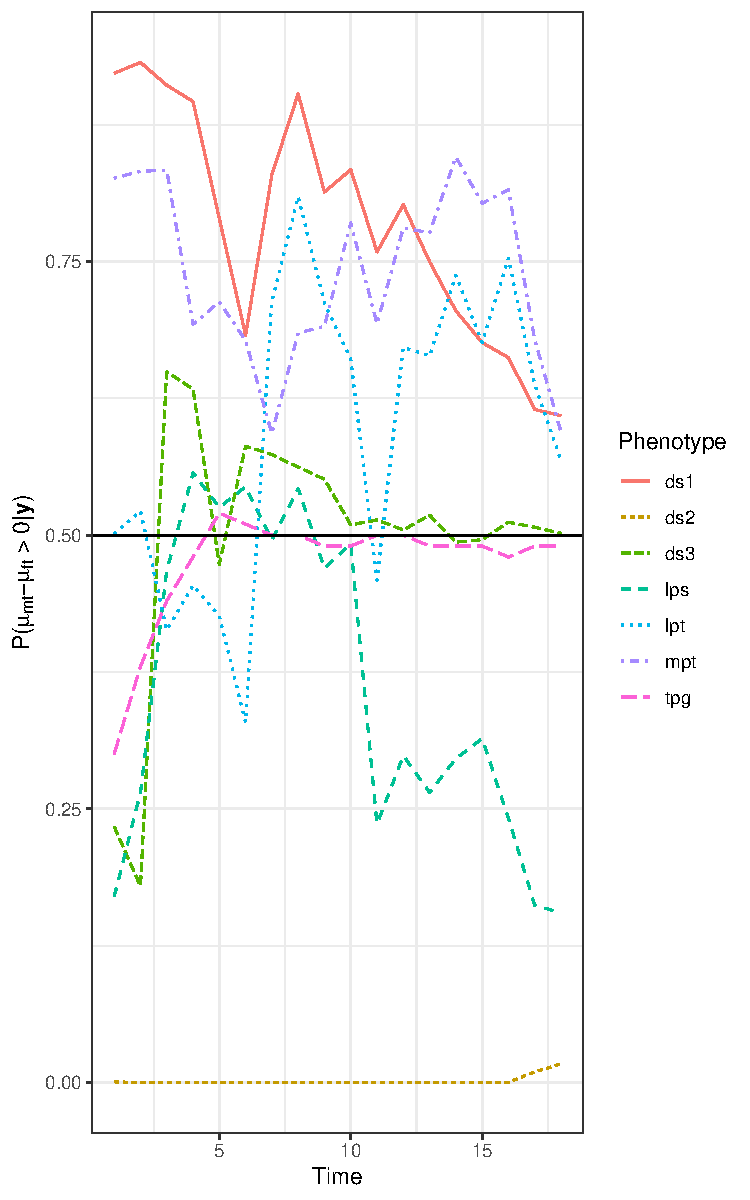
\includegraphics{../Figures/SD_Figures/post_probs_armor} 

}

\caption{Posterior probability of positive sexual dimorphism for armor traits}\label{fig:unnamed-chunk-2}
\end{figure}

\label{fig:post_probs_armor}

\begin{figure}

{\centering 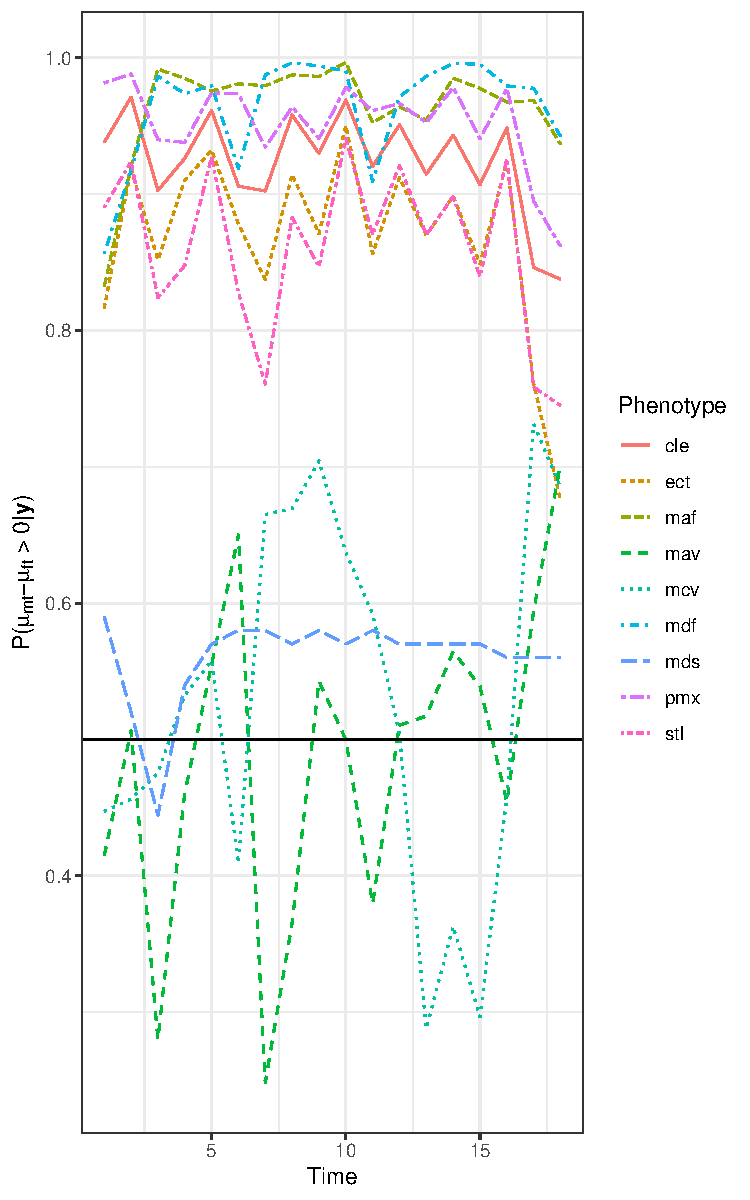
\includegraphics{../Figures/SD_Figures/post_probs_nonarmor} 

}

\caption{Posterior probability of positive sexual dimorphism for non-armor traits}\label{fig:unnamed-chunk-3}
\end{figure}

\label{fig:post_probs_nonarmor}

Then, to test our prediction that ecological release should result in an
increase in sexual dimorphism through time, we calculated Kendall's
\(\tau\) coefficient for each trait (Kendal
(\protect\hyperlink{ref-KendallsTau}{1938})). Kendall's \(\tau\)
assesses the ordinal association between a set of bivariate
observations, where \(\tau > 0\) indicates concordance between the
observations (i.e., as \(x\) increases, \(y\) also tends to increase;
here,\(x\) is time and \(y\) is sexual dimorphism.) Kendall's \(\tau\)
varies between -1 and 1, and can be thought of as behaving like a
correlation. Values farther from zero indicate a stronger relationship.

\(\boldsymbol{\tau}_k = \{\tau_{k,r}: r = 1,\cdots,R\}\) for trait \(k\)
where \(\tau_r\) is the estimate of the Kendall's \(\tau\) correlation
for \(\mu_{k,m,t_i} - \mu_{k,f,t_i}\) versus time \(t_i\) for the
\(r^{th}\) MCMC sample from the posterior distribution.
\textcolor{red}{Matt, I think there's an absolute value problem here. Dimorphism can increase of M-F gets more positive or more negative. I've indicated that in the text below, but I could use some help refininig the explanation -YS}
For each trait, the proportion of values in \(\boldsymbol{\tau}_k\) that
are greater than 0 (\(\frac{1}{R} \sum_{r=1}^R I(\tau_{k,r} > 0)\)) may
indicate that males have gotten relatively larger than females,
indicating more pronounced dimorphism. For each trait, the proportion of
values in \(\boldsymbol{\tau}_k\) that are less than 0
(\(\frac{1}{R} \sum_{r=1}^R I(\tau_{k,r} < 0)\)) may indicate that
females have gotten relatively larger than males, indicating more
pronounced dimormphism.

\hypertarget{sec:results}{%
\section{Results}\label{sec:results}}

The extant data used here consist of a total of 367 specimens all with
known sex (Table S1). Of these, there are 202 and 165 female and male
specimens, respectively.

\hypertarget{missing-data-imputation}{%
\subsection{Missing Data Imputation}\label{missing-data-imputation}}

\textcolor{red}{Greg, WE NEED RESULTS SECTION DESCRIBING THE RESULTS OF AKHIL'S MULTIPLE IMPUTATION, BOTH THE TESTS OF HOW WELL THE MODEL WORKED CLASSIFYING MODEL SAMPLES, AND SUMMARY STATISTICS OF FOSSIL IMPUTATION RESULTS -YS}

\hypertarget{sexual-dimorphism}{%
\subsection{Sexual Dimorphism}\label{sexual-dimorphism}}

Table \ref{tab:prob0-table} shows the posterior probability of the
differences in the means between male and female specimens at each time
point. Probabilities near 0.5 indicate very little difference in the
means whereas probabilities far from 0.5 indicate sexual dimorphism with
values of 0 and 1 indicating larger mean values for females and males,
respectively. These results are shown graphically in figure
\ref{fig:prob0-plot}.

Figure \ref{fig:mu-diff-plot} shows the posterior mean difference for
males versus females (values above 0 indicate means that were greater
for males versus females). The full posterior distributions over time
for all traits are shown in the appendix.

\hypertarget{changes-over-time}{%
\subsection{Changes over time}\label{changes-over-time}}

We can also assess the strength of the dimorphism by calculating the
proportion of posterior samples that are greater than a prespecified
threshold \textcolor{red}{(0.5??, idk what this could be.) -MS}

Table \ref{tab:auc-table} shows the probability that the posterior
distribution of the differences in the mean is greater than the
posterior distribution of the differences at the first time point.
Values near 0.5 indicate very little difference between the
distributions whereas values closer to 0 and 1 indicate changes in the
distributions with values of 1 meaning the difference in means has
shifted towards males having a larger mean and values of 0 indicating
the difference in means has shifted towards larger means in females.
These results are shown graphically in figure \ref{fig:AUC-plot}.

\hypertarget{sec:conclusions}{%
\section{Discussion, Future work and
conclusions}\label{sec:conclusions}}

We predicted that release from predators would result in niche expansion
and increased sexual dimorphism, based on several studies of modern
stickleback. For example, in lakes where sculpin competitors are absent
and stickleback (Roesti et al.~2023) See Spoljaric and Reimchen 2008,
page 512 right column for references and discussion of differences
between benthic males and limnetic females. Male stickleback are benthic
and littoral (Wootton 1976)\ldots. Reimchen papers in general good for
this section. Moreover, tooth wear data from the lineage II sequence
suggest that individuals in this lineage began eating more planktonic
prey over time, expanding toward an open-water niche from the benthic,
bottom-feeding niche they started with (Purnell et al.~2007). That this
expansion into open water by lineage II coincided with armor reduction
is further indicative of a limnetic system with fewer salmonid
piscivores (Schluter and McPhail
(\protect\hyperlink{ref-SchluterandMcPhail1992}{1992}); Vamosi and
Schluter (\protect\hyperlink{ref-VamosiandSchluter2004}{2004}); Roesti
et al. (\protect\hyperlink{ref-Roestietal2023}{2023})).

\hypertarget{sec:acknowl}{%
\section{Acknowledgements}\label{sec:acknowl}}

We thank O. Abughoush, S. Blain, A. Chaudhary, M. Islam, F. Joaquin, C.
Lawson-Weinert, R. Sullivan, J. Tien, M.P. Travis, and W. Shim for help
with data collection. We thank D. Schluter and S. Blain for loaning
specimens and sharing data. We thank K. Swagel and C. McMahan of the
Field Museum for assistance with specimen x-rays. This research was
supported by NSF grants BSR-8111013, EAR-9870337, and DEB-0322818, the
Center for Field Research (Earthwatch), and the National Geographic
Society (2869-84) to MAB. It was also supported by NSF grants
DEB-1456462 and EAR-2145830 to YES. And NSF DMS-2015374 (GJM)

\hypertarget{sec:datastatement}{%
\section{Data and Code Statement}\label{sec:datastatement}}

All code for reproducing the analyses in this paper is publicly
available at \url{https://github.com/Akhil-Ghosh/SticklebackProject}
\textcolor{red}{Is this true? Matt's code is at this GitHub page? -YS}

\hypertarget{sec:references}{%
\section{References}\label{sec:references}}

\hypertarget{sec:supplementary}{%
\section{Supplementary Material}\label{sec:supplementary}}

\hypertarget{refs}{}
\begin{CSLReferences}{1}{0}
\leavevmode\vadjust pre{\hypertarget{ref-Aguirreetal2014}{}}%
Aguirre, W E, K Walker, and S Gideon. 2014. {``Tinkering with the Axial
Skeleton: Vertebral Number Variation in Ecologically Divergent
Threespine Stickleback Populations.''} \emph{Biological Journal of the
Linnean Society} 113 (1): 204--19.

\leavevmode\vadjust pre{\hypertarget{ref-Baumgartneretal1988}{}}%
Baumgartner, J V, M A Bell, and P H Weinberg. 1988. {``Body Form
Differences Between the Enos Lake Species Pair of Threespine
Sticklebacks (Gasterosteus Aculeatus Complex).''} \emph{Canadian Journal
of Zoology} 66 (2): 467--74.

\leavevmode\vadjust pre{\hypertarget{ref-Bell2009}{}}%
Bell, M A. 2009. {``Implications of a Fossil Stickleback Assemblage for
Darwinian Gradualism.''} \emph{Journal of Fish Biology} 75 (8):
1977--99.

\leavevmode\vadjust pre{\hypertarget{ref-Belletal1985}{}}%
Bell, M A, J V Baumgartner, and E C Oslon. 1985. {``Patterns of Temporal
Change in Single Morphological Characters of a Miocene Stickleback
Fish.''} \emph{Paleobiology} 11: 258--71.

\leavevmode\vadjust pre{\hypertarget{ref-Belletal1993}{}}%
Bell, M A, G Orti, J A Walker, and J P Koenings. 1993. {``Evolution of
Pelvic Reduction in Threespine Sticklebacks: A Test of Competing
Hypotheses.''} \emph{Evolution} 47: 906--14.

\leavevmode\vadjust pre{\hypertarget{ref-Belletal2006}{}}%
Bell, M A, M P Travis, and D M Blouw. 2006. {``Inferring Natural
Selection in a Fossil Threespine Stickleback.''} \emph{Paleobiology} 32
(4): 562--77.

\leavevmode\vadjust pre{\hypertarget{ref-Blain2022}{}}%
Blain, S A. 2022. \emph{Evolutionary Outcomes of Interactions Among
Phenotypes in Post-Glacial Lakes}. University of British Columbia,
Canada.

\leavevmode\vadjust pre{\hypertarget{ref-Bolnick2011}{}}%
Bolnick, D I. 2011. {``Sympatric Speciation in Threespine Stickleback:
Why Not?''} \emph{International Journal of Ecology} 2011: 1--15.

\leavevmode\vadjust pre{\hypertarget{ref-BolnickandDoebeli2003}{}}%
Bolnick, D I, and M Doebeli. 2003. {``Sexual Dimorphism and Adaptive
Speciation: Two Sides of the Same Ecological Coin.''} \emph{Evolution}
57 (11): 2433--49.

\leavevmode\vadjust pre{\hypertarget{ref-BolnickandLau2008}{}}%
Bolnick, D I, and O L Lau. 2008. {``Predictable Patterns of Disruptive
Selection in Stickleback in Postglacial Lakes.''} \emph{The American
Naturalist} 172 (1): 1--11.

\leavevmode\vadjust pre{\hypertarget{ref-Bowne1994}{}}%
Bowne, P S. 1994. {``Systematics and Morphology of the
Gasterosteiformes.''} In \emph{The Evolutionary Biology of the
Threespine Stickleback}, edited by M A Bell and S A Foster. Oxford, UK:
Oxford University Press.

\leavevmode\vadjust pre{\hypertarget{ref-Butleretal2007}{}}%
Butler, Sawyer, M A, and J B Losos. 2007. {``Sexual Dimorphism and
Adaptive Radiation in Anolis Lizards.''} \emph{Nature} 447 (7141):
202--5.

\leavevmode\vadjust pre{\hypertarget{ref-MICE}{}}%
Buuren, Stef van, and Karin Groothuis-Oudshoorn. 2011. {``Mice:
Multivariate Imputation by Chained Equations in r.''} \emph{Journal of
Statistical Software} 45 (3): 1--67.
\url{https://doi.org/10.18637/jss.v045.i03}.

\leavevmode\vadjust pre{\hypertarget{ref-Cerasonietal2024}{}}%
Cerasoni, J N, M A Bell, and Y E Stuart. 2024. {``Geology,
Microstratigraphy, and Paleontology of Truckee Formation Lacustrine
Diatomite Deposits Near Hazen, Nevada, USA, with Emphasis on Fossil
Stickleback Fish.''} \emph{PaleoBios} 41: 1--15.

\leavevmode\vadjust pre{\hypertarget{ref-Cooperetal2011}{}}%
Cooper, I A, R T Gilman, and J W Boughman. 2011. {``Sexual Dimorphism
and Speciation on Two Ecological Coins: Patterns from Nature and
Theoretical Predictions.''} \emph{Evolution} 65 (9): 2553--71.

\leavevmode\vadjust pre{\hypertarget{ref-DeLisleetal2018}{}}%
De Lisle, S P, S Paiva, and L Rowe. 2018. {``Habitat Partitioning During
Character Displacement Between the Sexes.''} \emph{Biology Letters} 14:
20180124.

\leavevmode\vadjust pre{\hypertarget{ref-DeLisleandRowe2015}{}}%
De Lisle, S P, and L Rowe. 2015. {``Ecological Character Displacement
Between the Sexes.''} \emph{The American Naturalist} 186: 693--707.

\leavevmode\vadjust pre{\hypertarget{ref-DeLisleandRowe2017}{}}%
---------. 2017. {``Disruptive Natural Selection Predicts Divergence
Between the Sexes During Adaptive Radiation.''} \emph{Ecology and
Evolution} 7: 3590--3601.

\leavevmode\vadjust pre{\hypertarget{ref-Godfreyetal1993}{}}%
Godfrey, L R, S K Lyon, and M R Sutherland. 1993. {``Sexual Dimorphism
in Large-Bodied Primates: The Case of the Subfossil Lemurs.''}
\emph{American Journal of Physical Anthropology} 90: 315--34.

\leavevmode\vadjust pre{\hypertarget{ref-Hendryetal2009}{}}%
Hendry, A P, D I Bolnick, D Berner, and C L Peichel. 2009. {``Along the
Speciation Continuum in Sticklebacks.''} \emph{Journal of Fish Biology}
75 (8): 2000--2036.

\leavevmode\vadjust pre{\hypertarget{ref-Herrmannetal2021}{}}%
Herrmann, N C, J T Stroud, and J B Losos. 2021. {``The Evolution of
'Ecological Release' into the 21st Century.''} \emph{Trends in Ecology
and Evolution} 36 (3): 206--15.

\leavevmode\vadjust pre{\hypertarget{ref-HoneandMallon2017}{}}%
Hone, D W E, and J C Mallon. 2017. {``Protracted Growth Impedes the
Detection of Sexual Dimorphism in Non-Avian Dinosaurs.''}
\emph{Palaeontology} 60 (4): 535--45.

\leavevmode\vadjust pre{\hypertarget{ref-Huntetal2008}{}}%
Hunt, G, M A Bell, and M P Travis. 2008. {``Evolution Toward a New
Adaptive Optimum: Phenotypic Evolution in a Fossil Stickleback
Lineage.''} \emph{Evolution} 62 (3): 700--710.

\leavevmode\vadjust pre{\hypertarget{ref-Huxley1932}{}}%
Huxley, J S. 1932. \emph{Problems of Relative Growth}. L. MacVeagh.

\leavevmode\vadjust pre{\hypertarget{ref-KendallsTau}{}}%
Kendal, M G. 1938. {``{A new measure of rank correlation}.''}
\emph{Biometrika} 30 (June): 81--93.
\url{https://doi.org/10.1093/biomet/30.1-2.81}.

\leavevmode\vadjust pre{\hypertarget{ref-KoscinskiandPietraszewski2004}{}}%
Koscinski, K, and S Pietraszewski. 2004. {``Methods to Estimate Sexual
Dimorphism from Unsexed Samples: A Test with Computer Generated
Samples.''} \emph{Przeglad Antropologiczny - Anthropological Review} 67:
33--55.

\leavevmode\vadjust pre{\hypertarget{ref-little2002statistical}{}}%
Little, R. J. A., and D. B. Rubin. 2002. \emph{Statistical Analysis with
Missing Data}. Wiley Series in Probability and Mathematical Statistics.
Probability and Mathematical Statistics. Wiley.
\url{http://books.google.com/books?id=aYPwAAAAMAAJ}.

\leavevmode\vadjust pre{\hypertarget{ref-Mallon2017}{}}%
Mallon, J C. 2017. {``Recognizing Sexual Dimorphism in the Fossil
Record: Lessons from Nonavian Dinosaurs.''} \emph{Paleobiology} 43 (3):
495--507.

\leavevmode\vadjust pre{\hypertarget{ref-ParentandCrespi2009}{}}%
Parent, C E, and B J Crespi. 2009. {``Ecological Opportunity in Adaptive
Radiation of Galapagos Endemic Land Snails.''} \emph{The American
Naturalist} 174: 898--905.

\leavevmode\vadjust pre{\hypertarget{ref-PfennigandPfennig2012}{}}%
Pfennig, D W, and K S Pfennig. 2012. \emph{\href{}{Evolution's Wedge:
Competition and the Origins of Diversity}}. University of California
Press, Berkeley, USA.

\leavevmode\vadjust pre{\hypertarget{ref-Reimchen1994}{}}%
Reimchen, T E. 1994. {``Predators and Morphological Evolution in
Threespine Stickleback.''} In \emph{The Evolutionary Biology of the
Threespine Stickleback}, edited by M A Bell and S A Foster. Oxford, UK:
Oxford University Press.

\leavevmode\vadjust pre{\hypertarget{ref-ReimchenandNosil2004}{}}%
Reimchen, T E, and P Nosil. 2004. {``Variable Predation Regimes Predict
the Evolution of Sexual Dimorphism in a Population of Threespine
Stickleback.''} \emph{Evolution} 58 (6): 1274--81.

\leavevmode\vadjust pre{\hypertarget{ref-Roestietal2023}{}}%
Roesti, M, J S Groh, S A Blain, M Huss, P Rassias, D I Bolnick, Y E
Stuart, C L Peichel, and D Schluter. 2023. {``Species Divergence Under
Competition and Shared Predation.''} \emph{Ecology Letters} 26: 111--23.

\leavevmode\vadjust pre{\hypertarget{ref-Saittaetal2020}{}}%
Saitta, T, M T Stockdale, N R Longrich, V Bonhomme, M J Benton, I C
Cuthill, and P J Makovicky. 2020. {``An Effect Size Statistical
Framework for Investigating Sexual Dimorphism in Non-Avian Dinosaurs and
Other Extinct Taxa.''} \emph{Biological Journal of the Linnean Society}
131 (2): 231--73. \url{https://doi.org/10.1093/biolinnean/blaa105}.

\leavevmode\vadjust pre{\hypertarget{ref-Schindelinetal2012}{}}%
Schindelin, J, I Arganda-Carreras, E Frise, V Kaynig, M Longair, T
Pietzsch, S Preibisch, C Rueden, S Saalfeld, and B Schmid. 2012.
{``Fiji: An Open-Source Platform for Biological-Image Analysis.''}
\emph{Nature Methods} 9: 976--682.

\leavevmode\vadjust pre{\hypertarget{ref-SchluterandMcPhail1992}{}}%
Schluter, D, and J D McPhail. 1992. {``Ecological Character Displacement
and Speciation in Sticklebacks.''} \emph{The American Naturalist} 140
(1): 85--108.

\leavevmode\vadjust pre{\hypertarget{ref-Schoener1968}{}}%
Schoener, T W. 1968. {``The Anolis Lizards of Bimini: Resource
Partitioning in a Complex Fauna.''} \emph{Ecology} 29: 704--26.

\leavevmode\vadjust pre{\hypertarget{ref-Shine1989}{}}%
Shine, R. 1989. {``Ecological Causes for the Evolution of Sexual
Dimorphism: A Review of the Evidence.''} \emph{The Quarterly Review of
Biology} 64 (4): 419--61.

\leavevmode\vadjust pre{\hypertarget{ref-Siddiquietal2024}{}}%
Siddiqui, R, S Swank, A Ozark, F Joaquin, M P Travis, C D McMahan, M A
Bell, and Y E Stuart. 2024. {``Inferring the Evolution of Reproductive
Isolation in a Lineage of Fossil Threespine Stickleback, Gasterosteus
Doryssus.''} \emph{Proceedings of the Royal Society B} 291: 20240337.

\leavevmode\vadjust pre{\hypertarget{ref-Stuartetal2021}{}}%
Stuart, Y E, J W Sherwin, A Kamath, and T Veen. 2021. {``Male and Female
Anolis Carolinensis Maintain Their Dimorphism Despite the Presence of
Novel Interspecific Competition.''} \emph{Evolution} 75 (11): 2708--16.

\leavevmode\vadjust pre{\hypertarget{ref-Stuartetal2020}{}}%
Stuart, Y E, M P Travis, and M A Bell. 2020. {``Inferred Genetic
Architecture Underlying Evolution in a Fossil Stickleback Lineage.''}
\emph{Nature Ecology and Evolution} 4 (11): 1549--57.

\leavevmode\vadjust pre{\hypertarget{ref-Stuartetal2017}{}}%
Stuart, Y E, T Veen, J N Weber, D Hanson, M Ravinet, B K Lohman, C J
Thompson, et al. 2017. {``Contrasting Effects of Environment and
Genetics Generate a Continuum of Parallel Evolution.''} \emph{Nature
Ecology and Evolution} 1 (6): 158.

\leavevmode\vadjust pre{\hypertarget{ref-OUProcess}{}}%
Uhlenbeck, G E, and L S Ornstein. 1930. {``On the Theory of the Brownian
Motion.''} \emph{Phys. Rev.} 36 (September): 823--41.
\url{https://doi.org/10.1103/PhysRev.36.823}.

\leavevmode\vadjust pre{\hypertarget{ref-VamosiandSchluter2004}{}}%
Vamosi, S M, and D Schluter. 2004. {``Character Shifts in the Defensive
Armor of Sympatric Sticklebacks.''} \emph{Evolution} 58: 376--85.

\leavevmode\vadjust pre{\hypertarget{ref-Vojeetal2022}{}}%
Voje, K L, M A Bell, and Y E Stuart. 2022. {``Evolution of Static
Allometry and Constraint on Evolutionary Allometry in a Fossil
Stickleback.''} \emph{Journal of Evolutionary Biology} 35 (3): 423--38.

\leavevmode\vadjust pre{\hypertarget{ref-Vojeetal2014}{}}%
Voje, K L, T F Hansen, C K Egset, G H Bolstad, and C Pelabon. 2014.
{``Allometric Constraints and the Evolution of Allometry.''}
\emph{Evolution} 68: 866--85.

\leavevmode\vadjust pre{\hypertarget{ref-ZhouReiter2010}{}}%
Zhou, X, and J Reiter. 2010. {``A Note on Bayesian Inference After
Multiple Imputation.''} \emph{The American Statistician} 64 (2):
159--63.

\end{CSLReferences}

\end{document}
